\documentclass{midl} % Include author names

% The following packages will be automatically loaded:
% jmlr, amsmath, amssymb, natbib, graphicx, url, algorithm2e
% ifoddpage, relsize and probably more

\jmlrvolume{-- Under Review}
\jmlryear{2027}
\jmlrworkshop{Full Paper -- MIDL 2027 submission}
\editors{Under Review for MIDL 2027}

\title[Short Title]{Full Title of Article}

% Single-blind: author names are revealed at submission.
% NOTE: the author list is FINAL at submission time -- no additions,
% removals or reordering after the deadline.
\midlauthor{\Name{Jungro Lee\nametag{$^{1}$}} \Email{firstauthor@ucl.ac.uk}\\
\Name{Petru Manescu\nametag{$^{1}$}} \Email{p.manescu@ucl.ac.uk}\\
\addr $^{1}$ Department of Computer Science, University College London, London, UK
}

\begin{document}

\maketitle

\begin{abstract}
% Abstract registration deadline: 2026-11-30 AoE.
The 21-gene recurrence score (RS) guides chemotherapy in early breast cancer, but the assay is
expensive and slow, which motivates predicting it from routine H\&E slides. Multiple-instance
learning on tile embeddings is the usual approach, but it encodes each tile independently and
does not model how individual cells are arranged. We therefore represent tissue as cell graphs,
built from HoVer-Net nuclei joined by Delaunay triangulation, and combine a graph neural network
on these graphs with a pathology foundation-model image branch through a learned gate, so that
the model can draw on both. Whereas earlier methods use the whole slide, we limit each slide
to $N$ regions of 1\,mm$^2$ and vary $N$ from 2 to 16. On TCGA-BRCA (1,038 patients) the gated
model reaches an AUROC of 85.1 with only two regions, and more regions change it by at most 1.2
points. On two external cohorts, applied without retraining, it stops improving at $N=4$ on
CPTAC-BRCA (AUROC 85.1) and at $N=8$ on UCH (75.5), so a few square millimetres of tissue are
enough. Finally, we relate interpretable descriptors of
the cell graphs to the RS. In all three cohorts the strongest correlate is the variability of
neoplastic nuclear size, a marker of nuclear pleomorphism.
\end{abstract}

\begin{keywords}
% comma separated
\end{keywords}

% =====================================================================
% Page budget (main text limit: 10 pages, excluding references,
% acknowledgements and appendix).
%   Introduction ............ 1.5 p
%   Related Work ............ 0.5 p
%   Methods ................. 2.0 p
%   Experiments and Results . 4.0 p
%   Discussion .............. 1.0 p
%   Conclusion .............. 0.3 p
% Reviewers are not obliged to read the appendix: anything that
% determines the evaluation must sit inside the 10 main pages.
% =====================================================================

\section{Introduction}
\label{sec:introduction}

Most breast cancers are found at an early stage, they are also hormone receptor-positive and
human epidermal growth factor receptor 2-negative (HR+/HER2$-$). These patients have surgery
and then endocrine therapy. The remaining question is whether to add chemotherapy. Only a
minority of them benefit from it, and the rest take on its side effects for nothing. Multi-gene
assays were therefore built to estimate the risk of recurrence from tumour gene expression. The
most widely used one is the 21-gene recurrence score (RS) \citep{paik2004, sparano2018}. The
assay works, but it is costly, which takes several thousand pounds per patient. It consumes
tumour tissue, of which result also arrives one to two weeks after a pathologist has already read
the haematoxylin and eosin (H\&E) slide. A model that predicts the RS from that slide would
not replace the assay, but it could instead triage which patients are sent for genomic testing,
and it would cost no extra tissue and no extra waiting. This is possible because two gene
groups dominate the score, namely proliferation and oestrogen signalling, which leave visible
traces in nuclear shape and in tissue architecture \citep{paik2004, elston1991}. These molecular
readouts have already been recovered from H\&E before. Examples include driver mutations
\citep{coudray2018}, microsatellite instability \citep{kather2019} and bulk expression
\citep{schmauch2020}. For the RS itself, hand crafted nuclear shape features
\citep{whitney2018} and deep learning \citep{howard2024} have both been tried.

Predicting tasks from a whole-slide image (WSI) runs first into size. A slide scanned at
$40\times$ spans on the order of $10^5 \times 10^5$ pixels and it also carries a single label,
and that label belongs to no particular region. Multiple instance learning (MIL) is the
standard answer to this. First, the slide becomes a bag of patches and each patch is encoded on its own.
A permutation invariant pooling function then turns the bag into one slide representation
\citep{dietterich1997, ilse2018, campanella2019}. The patch encoder has improved steadily
inside this formulation. It moved from ImageNet-pretrained convolutional networks
\citep{he2016, lu2021} to self-supervised pathology encoders, and then to foundation models
trained on $10^5$--$10^6$ slides \citep{chen2024, filiot2023}. The patch budget has not had
the same attention. Some pipelines tile the tissue exhaustively \citep{campanella2019, lu2021}.
Others sample $10^3$--$10^4$ tiles per slide \citep{courtiol2018, wulczyn2020}. 

A second limit is representation of molecular functions within the image. Pooling over patch embeddings throws away where the
patches were. Therefore, a patch embedding also describes local texture rather than the individual cells
and how they relate \citep{ilse2018, pati2022}. Graph neural networks (GNNs) were brought into
computational pathology to put this structure back. They are used at two granularities. In the
first, patches are the nodes and spatial adjacency gives the edges, as in SlideGraph+
\citep{lu2022} and Patch-GCN \citep{chen2021}. Second, each segmented nucleus become a
node and it carries a morphometric descriptor, which is joined to the nuclei near it
\citep{zhou2019, pati2022}. The model then reads tissue architecture directly instead of
inferring it from texture. A pathologist grades nuclear size, chromatin
density, crowding and tubule formation, and in a cell graph these are explicit properties
rather than latent directions in an embedding.

We combine the two views, and we ask how much tissue a model actually needs to see. Each slide
is reduced to a small number of pathches $N$ of tissue regions of $1 \times 1$\,mm ($4096$ pixels at
$0.25\,\mu$m/px). HoVer-Net \citep{graham2019} segments the nuclei inside a region. Those
nuclei form one cell graph that spans the whole region, with morphometric descriptors as node
features. The region is also split into sixteen tiles, and a frozen UNI2-h encoder embeds
each one. A learned gate fuses the graph embedding with those tile embeddings, and the region
vectors are then aggregated to the slide. We hold the architecture fixed and vary $N$ from 2
to 16. We evaluate on The Cancer Genome Atlas (TCGA) and on two external cohorts. RS prediction
saturates at small area, which is about $4\,\mathrm{mm}^2$ of tissue per slide, far below the
budgets used in the literature. From this, we found that the signal that matters for the RS is therefore not limited by
spatial coverage. It is no longer how much of the slide to
process, but which morphological properties carry the signal. Therefore, we address the second question
by relating graph morphology and cell-type composition to the recurrence score itself.

Our contributions are as follows.
\begin{itemize}
\item A region level dual branch model is designed with gated module to reflect both morphological features' relation and spatial feature of the image. 
\item A controlled study of the region budget, with $N \in \{2,4,8,16\}$ nested regions per
  slide was conducted. 
\item An analysis of which graph morphology features and cell types are associated with the
  recurrence score was conducted to identify where the predictive signal resides, not only how
  much tissue is needed to find it.
\end{itemize}
\section{Related Work}
\label{sec:related-work}

\paragraph{Nuclear segmentation: HoVer-Net.}
HoVer-Net \citep{graham2019} describes individual nuclei in histopathology image. It is consisted of a single encoder with three
decoder branches. One branch segments nuclear pixels, and a second regresses the horizontal and
vertical distances from each pixel to the centre of mass of its nucleus, which lets
the model split nuclei that touch. Lastly, a third assigns each instance a type. We use the weights
trained on PanNuke \citep{gamper2020}, a dataset of 205,343 labelled nuclei drawn from 19
tissue types and annotated into five classes: neoplastic, non-neoplastic epithelial,
inflammatory, connective or soft tissue, and dead. For comparison, the dataset used in the
original HoVer-Net paper held roughly 24,000 labelled nuclei from a single tissue type, so the
PanNuke weights transfer far better across organs. The output per nucleus is a contour, a
centroid, a class and a confidence.  Cell graphs in pathology are commonly built on them, as in CGC-Net \citep{zhou2019} and
HACT-Net \citep{pati2022}.

\paragraph{Patch encoding: UNI2-h.}
UNI \citep{chen2024} describes whole patches instead of single cells. It is a vision
transformer trained with DINOv2 \citep{oquab2024}, so no labels are used. The model learns
tissue features in two ways. It matches different views of the same image, and it fills in
masked regions from their surroundings. UNI2-h, the variant we use, is a ViT-H/14 of roughly
681M parameters. It was trained on more than 200 million patches from over 350,000 slides. Its
pretraining is documented not to include TCGA, which keeps our TCGA evaluation uncontaminated.
In an independent benchmark it ranked near the top across slide and patch level tasks
\citep{campanella2025}. The output is one embedding vector per patch. Such frozen embeddings
now serve as the instance features in most MIL pipelines \citep{lu2021, filiot2023}. 

\paragraph{Super-resolution: Swin2SR.}
Our cohorts are not scanned at the same magnification, and HoVer-Net is sensitive to this.
Nuclei that touch cannot be separated when they occupy too few pixels, which force us to upsample
the lower-magnification cohort before segmentation, using Swin2SR \citep{conde2022}. Swin2SR
is a transformer built on Swin V2 blocks \citep{liu2022}. It computes self-attention inside
local windows, and it shifts those windows between consecutive layers. This captures context
across windows while keeping the cost linear in the number of pixels. The $\times 4$ variant
we use is trained on DF2K, a collection of natural images, with bicubically downsampled inputs
and an $\ell_1$ pixel loss. However, it is therefore a general-purpose model and has seen no
histopathology. That turns out to be acceptable in this paper, \citet{juhong2023} report that
transformer-based super-resolution transfers to H\&E without retraining, at only a modest
cost in downstream segmentation. 

\paragraph{Message passing over cell graphs.}
A graph neural network (GNN) updates each node from its neighbours. We write $h^{(l)}_i$ for the
embedding of node $i$ at layer $l$ and $\mathcal{N}(i)$ for its neighbourhood. We use the graph
convolutional network (GCN) \citep{kipf2017}, which applies a symmetric normalised convolution,
\begin{equation}
\label{eq:gcn}
h^{(l+1)}_{i} = \sigma\!\left( \sum_{j \in \mathcal{N}(i) \cup \{i\}}
\frac{W^{(l)} h^{(l)}_{j}}{\sqrt{\hat{d}_i \hat{d}_j}} \right),
\end{equation}
where $\hat{d}_i$ is the degree of node $i$ including its self-loop. The normalising term
damps the degree signal without removing it, so a node is described mainly by the morphology
of its neighbours rather than by how many it has. GCN is also the simplest and cheapest of the
common operators, which matters when one graph holds several thousand nuclei.

\paragraph{Edge derivation in cell graphs.}
The edge rule decides which notion of neighbourhood the graph encodes. We use Delaunay
triangulation, which joins nuclei whose Voronoi cells share a boundary. The result is a
connected planar graph that approximates physical cell contact, and it is the usual choice when
the graph should represent tissue architecture rather than mere proximity
\citep{gunduz2004, lu2022}. Its decisive property here is that it needs no scale parameter.
The common alternatives each fix one: a radius rule ties connectivity to a distance tuned to one
cohort's nuclear spacing \citep{pati2022}, and a $k$-nearest-neighbour rule fixes $k$ in advance
\citep{zhou2019}. Delaunay therefore transfers unchanged between cohorts whose cellular density
differs.

\paragraph{Predicting the recurrence score from H\&E.}
The 21-gene recurrence score summarises the expression of sixteen cancer-related genes. These
are normalised against five reference genes and aggregated into four functional group scores
\citep{paik2004}. The unscaled score is a fixed weighted sum of those groups,
\begin{equation}
\label{eq:rs}
\begin{split}
\mathrm{RS}_{u} = \;&+0.47\,\mathrm{HER2} - 0.34\,\mathrm{ER} + 1.04\,\mathrm{Prolif}
+ 0.10\,\mathrm{Invasion} \\
&+ 0.05\,\mathrm{CD68} - 0.08\,\mathrm{GSTM1} - 0.07\,\mathrm{BAG1},
\end{split}
\end{equation}
where each term is the expression score of a gene group (ER: oestrogen receptor group; Prolif:
proliferation group) or of a single gene. The HER2 and proliferation group scores are
thresholded from below before they enter \equationref{eq:rs}. The result is then rescaled to
the reported $0$--$100$ range as
$\mathrm{RS} = \min\{100, \max\{0,\, 20(\mathrm{RS}_{u} - 6.7)\}\}$ \citep{paik2004}. In this equation, the proliferation group carries the largest positive weight, and the
oestrogen group carries the only substantial negative one. This is what makes the score
accessible from morphology at all. Proliferation is visible as enlarged nuclei, dense
chromatin, mitotic figures and crowding. Oestrogen signalling instead accompanies a
differentiated, tubule-forming architecture with uniform nuclei \citep{elston1991}.  Thanks to these properties, molecular
readouts have accordingly been recovered from H\&E in several settings. Two previous studies address the recurrence score directly.
\citet{whitney2018} showed that hand-crafted nuclear shape features separate low- from
high-risk categories. \citet{howard2024} reported an area under the receiver operating
characteristic curve (AUROC) of 0.797 on the TCGA breast cancer cohort (TCGA-BRCA) with
patch-based deep learning. 

\section{Methods}
\label{sec:methods}

The pipeline turns one gigapixel slide into one risk estimate, and it does so in two halves.
The first half builds the input. A slide is reduced to $N$ tissue regions, those regions are
brought to a common resolution, their nuclei are segmented, each nucleus is given a
morphometric descriptor, and the nuclei of a region are joined into one cell graph. The second
half is the model. A graph branch encodes the cell graph of a region, an image branch encodes
the same region from its tiles, a learned gate fuses the two, attention over regions reduces a
slide to one vector, and a head produces the prediction. \sectionref{sec:cell-graph-construction}
covers the first half and \sectionref{sec:dual-branch-architecture} the second. The budget $N$
is the one quantity we vary, and \sectionref{sec:region-sampling-protocol} describes how.

\subsection{Cell Graph Construction}
\label{sec:cell-graph-construction}

First, regions are drawn. Tissue is separated from background glass by Otsu thresholding of a
low-resolution level of the slide. Candidate windows of $4096 \times 4096$ level-0 pixels
($1.02$\,mm on a side) are laid on a half-window stride. Windows with a tissue fraction below
0.6 are discarded, or below 0.3 if none survives, and $N$ non-overlapping windows are then
drawn at random with a seed fixed per slide. A region is the unit seen by both branches. It is
large enough to contain glandular and stromal architecture, yet small enough for a single cell
graph to cover it.

Second, resolution is harmonised. The three cohorts are scanned at different magnifications,
and HoVer-Net separates touching nuclei reliably only at the resolution it was trained for, so
we bring every region to a common effective $0.25\,\mu$m/px with the transformer-based
super-resolution model Swin2SR \citep{conde2022}. Slides scanned at $20\times$ (51 TCGA slides
and 144 of the 273 CPTAC-BRCA series) are cut at 2048 pixels and upsampled $\times 2$. The UCH
cohort is distributed only as $299$-pixel tiles at $\approx 10\times$, so a region is stitched
from a $4 \times 4$ block of adjacent tissue tiles, centre-cropped to 1024 pixels and upsampled
$\times 4$. Every region therefore enters segmentation with the same physical field of about
$1\,\mathrm{mm}^{2}$ and the same effective resolution.

To confirm that upsampling restores the structure HoVer-Net relies on, we take 20 native
$40\times$ TCGA regions from different slides (central 512\,$\mu$m), degrade them to $20\times$
and $10\times$ by area averaging, bring them back to $0.25\,\mu$m/px with Swin2SR (with the
pipeline's settings) or with bicubic interpolation, and match the HoVer-Net detections on each
version to those on the native image by centroid (one-to-one, within 4\,$\mu$m). The $\times 2$
path is almost lossless with either method (F1 0.98). On the $\times 4$ path, Swin2SR recovers
92\% of the nuclei with 90\% type agreement and keeps 97\% of the matched neoplastic nuclei
neoplastic. Bicubic interpolation misses 15\% of the nuclei and relabels a quarter of the
neoplastic ones, mostly as connective (\figureref{fig:sr-fidelity}, \tableref{tab:sr-fidelity}).
After Swin2SR the neoplastic fraction, on which the node features depend, is off by 4.9
percentage points on average, against 11.5 after bicubic interpolation.

% Data: Dissertation/Results/tables/sr_validation_{regions,summary}.csv
% (code/preprocessing/run_sr_validation.sh, code/model/sr_validation_eval.py)
% Figure: Dissertation/code/figures/latex/fig_sr_fidelity.py
\begin{figure}[htbp]
\floatconts
  {fig:sr-fidelity}
  {\caption{HoVer-Net on a TCGA region at $10\times$, after bicubic or Swin2SR $\times 4$ restoration, and at native $40\times$ (contour colour: cell type).}}
  {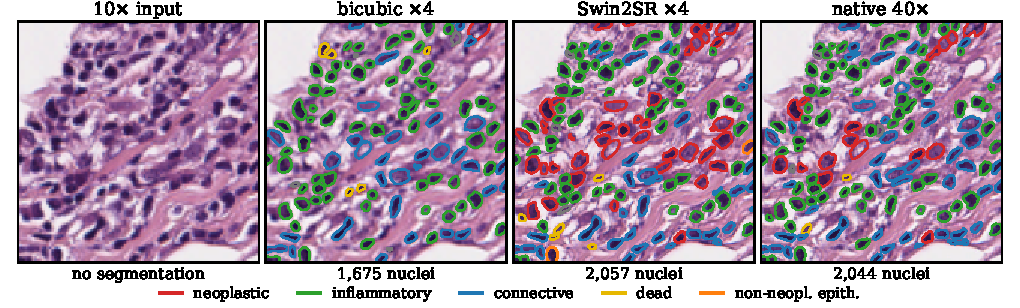
\includegraphics[width=\linewidth]{figures/fig_sr_fidelity.pdf}}
\end{figure}

\begin{table}[htbp]
\floatconts
  {tab:sr-fidelity}
  {\caption{Agreement with HoVer-Net on native $40\times$ over 20 TCGA regions (Count: restored / native nuclei; $\Delta$neo: error of the neoplastic fraction in points).}}
  {\small
  \begin{tabular}{llcccccc}
  \hline
  Input & Method & Count & Prec. & Rec. & F1 & Type & $\Delta$neo \\
  \hline
  $20\times$ & Bicubic $\times 2$  & 0.99 & 0.98 & 0.97 & 0.98 $\pm$ 0.02 & 0.97 & 1.1 \\
             & Swin2SR $\times 2$  & 1.01 & 0.98 & 0.99 & 0.98 $\pm$ 0.01 & 0.97 & 1.9 \\
  \hline
  $10\times$ & Bicubic $\times 4$  & 0.88 & 0.98 & 0.85 & 0.91 $\pm$ 0.04 & 0.80 & 11.5 \\
             & Swin2SR $\times 4$  & 0.98 & 0.95 & 0.92 & 0.93 $\pm$ 0.04 & 0.90 & 4.9 \\
  \hline
  \end{tabular}}
\end{table}

Third, nuclei are segmented. Each $1.02$\,mm region is passed whole through HoVer-Net
\citep{graham2019} with PanNuke-pretrained weights (tile mode with overlapping stitching, so
that nuclei on internal boundaries are not cut), which returns for every nucleus a centroid, a
polygonal contour, an axis-aligned bounding box, and one of six PanNuke cell types with its
confidence. How many nuclei a region holds differs by cohort: a TCGA region contains 3,971 on
average (median 3,855, interquartile range 2,286--5,198), against 4,122 in CPTAC-BRCA and
2,664 in UCH. Regions with too few nuclei to triangulate
are background, yield no graph, and are discarded.

Fourth, each nucleus becomes a node. Its feature is a $13$-dimensional morphometric descriptor
built entirely from the HoVer-Net output: the centroid (2), a one-hot encoding of the six
PanNuke classes (6), the type confidence (1), and four shape terms, namely log nuclear area,
log perimeter, bounding-box aspect ratio and convexity (4). The centroid and the shape terms
are $z$-scored within the region.

Fifth, the nodes are joined into edges. Edges are derived from the centroid coordinates by
Delaunay triangulation, which connects nuclei whose Voronoi cells are adjacent. One graph spans
the whole region, running straight across the boundaries of the sixteen tiles seen by the image
branch. The rule requires no scale parameter, so it
applies unchanged to cohorts whose nuclear density differs.

% Figure: Dissertation/code/figures/latex/fig_cohort_graphs.py
% \begin{figure}[htbp]
% \floatconts
%   {fig:cohort-graphs}
%   {\caption{HoVer-Net output and cell graphs in the three cohorts. One region per cohort, chosen
%   as the region whose nucleus count is closest to the cohort median, shown on the $192\,\mu$m
%   window with the most neoplastic nuclei. Top: nuclear contours coloured by HoVer-Net type.
%   Bottom: the Delaunay graph used for training, nodes coloured by type. Titles give the nucleus
%   count and the mean $\pm$ SD node degree of the whole region.}}
%   {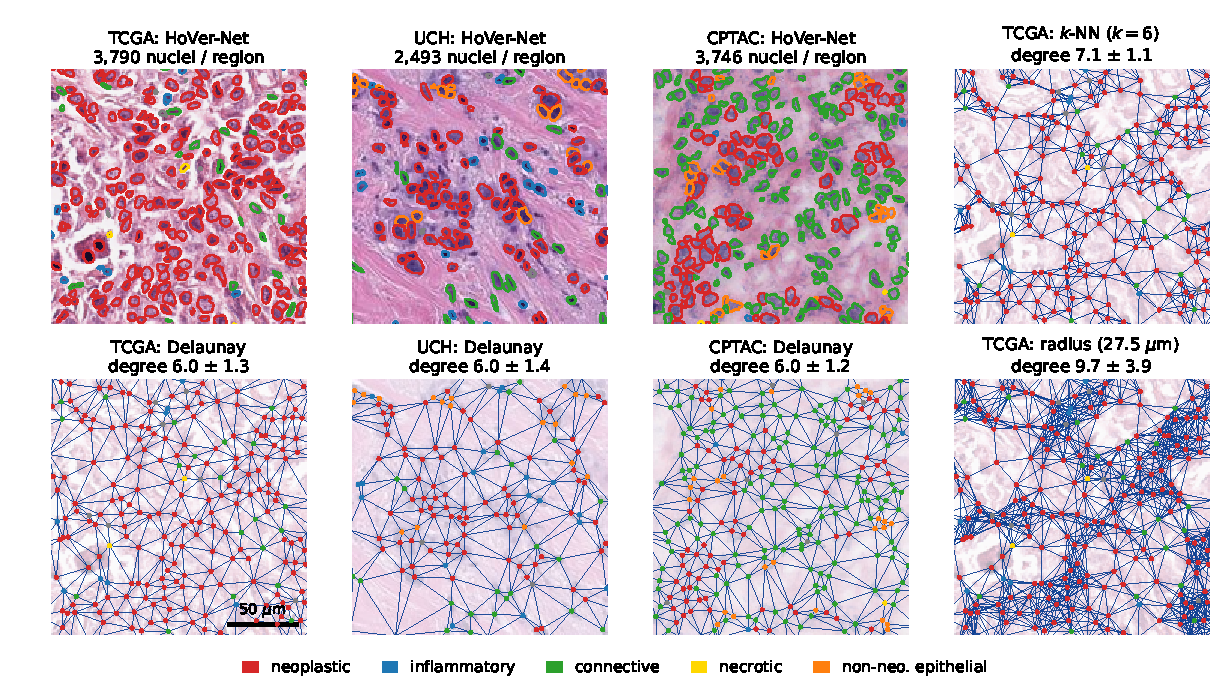
\includegraphics[width=0.8\linewidth]{figures/fig_cohort_graphs.pdf}}
% \end{figure}

\subsection{Dual-Branch Architecture}
\label{sec:dual-branch-architecture}

The model has five components, and the first two run in parallel over the same region.

First, the graph branch. The region graph is processed by a graph convolutional network (GCN)
\citep{kipf2017} of $L=3$ layers and width $d_g=128$, each layer followed by batch
normalisation, ReLU and dropout. Node embeddings $h_i$ are pooled by concatenating their mean
and element-wise maximum and projecting back to $d_g$,
\begin{equation}
\label{eq:region-readout}
z^{g}_{r} = \mathrm{LayerNorm}\!\left( \mathrm{ReLU}\!\left( W \left[ \tfrac{1}{|V_r|}
\textstyle\sum_{i \in V_r} h_i \;\big\|\; \max_{i \in V_r} h_i \right] \right) \right),
\end{equation}
where $V_r$ is the node set of region $r$. The readout retains both the typical nucleus and the
most extreme one, since a single highly abnormal nucleus can be diagnostically decisive.

Second, the image branch. The same region is divided into a $4 \times 4$ grid of 1024-pixel
tiles, and each tile is divided again into a $4 \times 4$ grid of 256-pixel views, so that
cell-level detail is not blurred away by the resizing UNI2-h \citep{chen2024} requires. Each
view is embedded by the frozen encoder, taking the class token concatenated with the mean patch
token (3072-d), and the sixteen view embeddings are averaged. Each tile vector is projected to
128 dimensions by LayerNorm, a linear map, ReLU and dropout. The sixteen tiles are then pooled
by gated attention \citep{ilse2018} and normalised, giving $z^{u}_{r}$.

Third, the two branches are fused at region level, before slide aggregation, by a single
learned scalar that scales the image branch against the normalised graph branch,
\begin{equation}
\label{eq:fusion}
z_{r} = \left[\, g \cdot z^{u}_{r} \;\big\|\; z^{g}_{r} \,\right],
\end{equation}
where $g$ is initialised at 1 and learned with the rest of the network. Both branch outputs are
layer-normalised, so $g$ is directly interpretable as the relative weight of the image branch.
A value $g>1$ means the image branch dominates and $g<1$ the cell graph, and we report it as a
result.

Fourth, the regions are aggregated with attention. The fused region vectors
$\{z_r\}_{r=1}^{N}$ of a slide are reduced to a single slide vector by gated attention pooling
\citep{ilse2018},
\begin{equation}
\label{eq:abmil}
z_{S} = \sum_{r} a_{r} z_{r}, \qquad
a_{r} = \frac{\exp\!\left( w^{\top} \left( \tanh(V z_{r}) \odot \sigma(U z_{r}) \right) \right)}
{\sum_{q} \exp\!\left( w^{\top} \left( \tanh(V z_{q}) \odot \sigma(U z_{q}) \right) \right)},
\end{equation}
where $\sigma$ is the logistic sigmoid. The weights $a_r$ can be read directly as region
importance, and inspected against the morphology of the regions they select.

Fifth, the head produces the prediction. The slide vector passes through LayerNorm, a linear
layer of width 64, ReLU and dropout into a single logit, trained on the binarised recurrence
score with a class-weighted binary cross-entropy,
\begin{equation}
\label{eq:loss}
\mathcal{L} = -\frac{1}{|B|} \sum_{S \in B} \Big[ \omega\, y_S \log \hat{p}_S
+ (1 - y_S) \log (1 - \hat{p}_S) \Big], \qquad \omega = \frac{n_{-}}{n_{+}},
\end{equation}
where $n_{+}$ and $n_{-}$ count the positive and negative training slides.

\subsection{Region Budget Protocol}
\label{sec:region-sampling-protocol}

The budget $N \in \{2, 4, 8, 16\}$ is the quantity we vary, which corresponds to roughly
2--16\,mm$^2$ of tissue per slide. The smallest setting is a deliberate anchor: $N=2$ matches
the segmentation budget of a conventional 32-patch pipeline ($2 \times 16$ tiles of 1024
pixels), so the model is still trained on a varied set of regions at the budget a patch-based
method would use. Region draws are nested, so every larger budget adds tissue to the smaller
one instead of replacing it. All other components are held fixed while $N$ is swept, so the
resulting curve isolates the dependence on coverage, and all regions of a slide are used in
training and inference.

\section{Experiments and Results}
\label{sec:experiments}

% ~4 pages total across the four subsections.

\subsection{Setup}
\label{sec:setup}

\paragraph{TCGA-BRCA (internal).}
Diagnostic formalin-fixed sections were streamed from the NCI Imaging Data Commons. 1,096
slides from 1,038 patients yield at least the first two regions. Labels are taken from the TCGA
clinical fields used by \citet{guo2026}. TCGA never ran the commercial Oncotype DX assay, so
the RS label is a research-grade score computed from bulk RNA sequencing of the 21 genes with
\equationref{eq:rs} \citep{paik2004}, thresholded at the 85th percentile of the HR+/HER2$-$
subset following \citet{howard2024}; this places 302 of the 1,038 patients in the high-risk
class.

\paragraph{UCH (external).}
The external cohort was collected at the University of Chicago Hospital (UCH) and, unlike
TCGA, carries clinically assayed Oncotype DX scores, which makes it the stricter test of
generalisation: the model must transfer across scanner, magnification and label provenance.
Slides with $\mathrm{RS} \geq 26$ are labelled high risk, giving 417 patients (472 slides, 77
high risk).

\paragraph{CPTAC-BRCA (external).}
The second external cohort is the Clinical Proteomic Tumor Analysis Consortium breast cancer
cohort (CPTAC-BRCA), a mix of $40\times$ and $20\times$ scans that, like TCGA, has no clinical
assay. We compute a surrogate RS from RNA sequencing:
$\log_2(\mathrm{TPM}+1)$ expression is normalised to the five reference genes, each gene is
min--max scaled to 0--15 across the cohort, and \equationref{eq:rs} is applied. A patient is
labelled high risk if $\mathrm{RS}_u \geq 12.24$, a cut-off fixed before any model was applied,
which places the same fraction of the 122 CPTAC patients with slides in the high-risk class as
in TCGA (28.7\%). 108 patients (263 slides, 34 high risk) yield regions.

\paragraph{Protocol.}
Internal evaluation follows the protocol of \citet{guo2026}: patient-level, label-stratified
five-fold cross-validation with a 7:1:2 train/validation/test ratio per fold. Their split
files are not released, so the splits are regenerated with the same protocol and a fixed seed,
and every model in this paper uses the same files. Every slide of a patient falls in the same
partition, and a patient's score is the mean of their slide probabilities. We report the mean
and standard deviation of the test AUROC over the five folds. The external cohorts are never
used for model selection: each configuration is applied as the ensemble of its five fold models
(mean of the five slide probabilities) without retraining or recalibration, and we report
patient-level AUROC with a 95\% confidence interval from 2,000 patient bootstrap resamples.

\paragraph{Random seeds.}
Seeds are fixed so that every comparison in this section is paired: the region draw of a slide
is seeded by the slide itself, the five splits are generated once and shared by all models, and
each fold has its own training seed. Every model, every budget $N$ and every rerun therefore
sees exactly the same tissue, so the TCGA band in \figureref{fig:auroc-vs-n} is the spread
across folds alone, and the spread caused by the region draw is measured separately below.

\paragraph{Region resampling.}
Because each slide contributes a single random draw, we test whether the results depend on which
regions were drawn. The sixteen regions of every slide are split into non-overlapping sets of
$N$ regions ($r_{kN},\dots,r_{(k+1)N-1}$), giving eight sets for $N=2$, four for $N=4$ and two
for $N=8$; set 0 is the draw used in \figureref{fig:auroc-vs-n}. The
gated model is retrained on every set with the same splits and seeds, and every trained model is
then tested on every set, both on the set it was trained on and on all others. This gives 64, 16
and 4 train-set/test-set combinations for $N = 2, 4, 8$ per cohort. Test patients are always the
held-out patients of the fold (or the external cohort), so only the tissue shown to the model
changes. A slide with no region in a test set is left out of that set only.

\paragraph{Training.}
Models are trained for 60 epochs with AdamW (learning rate $10^{-4}$, weight decay $10^{-3}$)
and cosine annealing to $10^{-6}$, a batch of four slides and dropout 0.3, on a single
GPU. The checkpoint with the best patient-level validation AUROC is evaluated on the test fold.
Graphs and tile embeddings are pre-computed, so training cost is dominated by the GNN and grows
linearly with $N$.

\paragraph{Cost measurement.}
All costs are measured on a single NVIDIA RTX 3090 Ti, with pre-processing throughput taken
from the extraction logs and the model itself timed on 120 TCGA slides that hold all sixteen
regions. Cost grows linearly with the region budget, and pre-processing dominates it: raising
$N$ from 2 to 16 takes a new slide from roughly one minute to a quarter of an hour
(\tableref{tab:cost}). A budget at the low end of the range is therefore the one worth having,
provided accuracy does not depend on it.

\begin{table}[htbp]
\floatconts
  {tab:cost}
  {\caption{Cost per slide against the region budget $N$ (gated model, RTX 3090 Ti).}}
  {\small
  \begin{tabular}{lcccccc}
  \hline
   & & & \multicolumn{2}{c}{Inference} & \multicolumn{2}{c}{Training} \\
  $N$ & Tissue (mm$^2$) & Nuclei & Total (min) & Model (ms) / Peak (GB) & ms & Peak (GB) \\
  \hline
  2  & 2.1  & 7,651  & 1.1--1.8  & 4.9 / 0.18 & 4.1  & 0.56 \\
  4  & 4.2  & 15,394 & 2.3--3.6  & 3.1 / 0.32 & 5.1  & 1.16 \\
  8  & 8.4  & 30,527 & 4.6--7.1  & 5.1 / 0.54 & 9.6  & 2.15 \\
  16 & 16.8 & 59,533 & 9.1--14.2 & 9.8 / 1.01 & 18.7 & 4.07 \\
  \hline
  \end{tabular}}
\end{table}

\subsection{Performance Across Region Budgets and Region Draws}
\label{sec:more-region-sampling}

\paragraph{Five-fold results.}
On TCGA the gated model is almost flat as $N$ grows (\figureref{fig:auroc-vs-n}): 85.1 at
$N=2$, 85.9 at $N=4$, 86.3 at $N=8$ and 85.5 at $N=16$. The whole range is 1.2 points, well
inside the fold-to-fold standard deviation of 3.1--4.2 points, so eight times more tissue buys
nothing that can be distinguished from noise. The image branch alone behaves the same way
(84.2 to 86.1, most of it between $N=2$ and $N=4$). The graph branch alone is the exception: it
rises from 76.2 to 80.4 and gains more from extra regions than either of the others, which
shows that additional tissue does change what a branch can learn even where the fused model
stops improving. It nevertheless stays 6 points behind the image branch at every budget. The
external cohorts repeat the pattern (\figureref{fig:auroc-vs-n}, centre and right). Gated RS reaches 85.1 on
CPTAC-BRCA at $N=4$ and 75.5 on UCH at $N=8$, and neither cohort improves beyond those budgets;
the gated model is ahead of the image branch by up to 3.8 points on CPTAC and within 1.5 points
of it on UCH.

% Figure: Dissertation/code/figures/latex/fig_auroc_vs_n_rs.py
\begin{figure}[htbp]
\floatconts
  {fig:auroc-vs-n}
  {\caption{RS AUROC (\%) against the region budget $N$; bands: $\pm 1$ SE across folds (TCGA) and 95\% bootstrap CI (external).}}
  {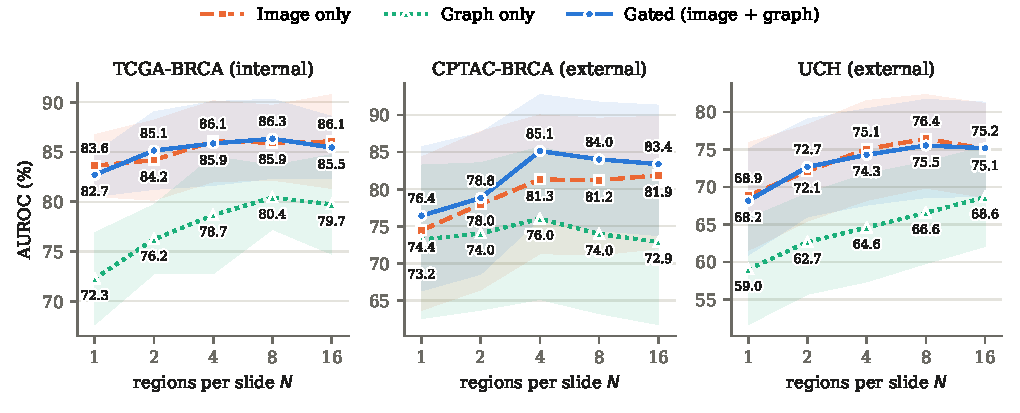
\includegraphics[width=\linewidth]{figures/fig_auroc_vs_n_rs.pdf}}
\end{figure}

\paragraph{Region draws.}
Training on a different draw of regions changes little. Retraining the gated model on every
non-overlapping set of $N$ regions and testing it on every set (\tableref{tab:resample}), the
spread on TCGA is 0.5--0.8 points, against 3.1--4.2 points across folds for the same model. The
mean over draws rises slightly from $N=2$ to $N=8$ (84.3 to 85.8), so the flat curve above is
not an artefact of one favourable draw, although that draw was indeed slightly favourable at
$N=2$ (85.1 against a mean of 84.3). Externally the spread is 0.9--2.3 points, and on CPTAC it
falls from 3.1 at $N=2$ to 0.9 at $N=4$.

\begin{table}[htbp]
\floatconts
  {tab:resample}
  {\caption{Gated AUROC (\%, mean $\pm$ SD) over all train-set/test-set combinations of non-overlapping region draws.}}
  {\small
  \begin{tabular}{lccc}
  \hline
  Cohort & $N=2$ & $N=4$ & $N=8$ \\
  \hline
  TCGA-BRCA  & 84.3 $\pm$ 0.8 & 85.2 $\pm$ 0.6 & 85.8 $\pm$ 0.5 \\
  CPTAC-BRCA & 81.6 $\pm$ 3.1 & 83.5 $\pm$ 0.9 & 83.2 $\pm$ 0.9 \\
  UCH        & 71.3 $\pm$ 2.3 & 73.2 $\pm$ 2.0 & 74.1 $\pm$ 1.4 \\
  \hline
  \end{tabular}}
\end{table}

% TODO: fold-wise paired Delta-AUROC (gated - image, N vs N=2) with bootstrap CI
%       (code/model/region_deltas.py) to back the saturation claim statistically

\subsection{Morphological Correlates of the Recurrence Score}
\label{sec:where-signal-lives}

To see which tissue properties carry the signal, we compute fourteen interpretable descriptors
of every $N=2$ region in physical units and relate their patient means to the recurrence score
(\figureref{fig:morph}). On TCGA the strongest correlate is the variability of neoplastic
nuclear size (area CV, $\rho = 0.47$), a measure of nuclear pleomorphism. High-RS tumours are
also denser and more neoplastic, with less connective tissue ($\rho = -0.28$). Architectural
descriptors are weaker ($|\rho| \le 0.15$). The area CV is also the strongest correlate on both
external cohorts (CPTAC-BRCA $\rho = 0.33$, UCH $\rho = 0.21$), and the only significant one on
CPTAC-BRCA. Because the node features are $z$-scored within each region, the
region-level spread of nuclear size is not directly available to the graph branch.

% Figure: Dissertation/code/figures/latex/fig_morph_heatmap_rs.py (data: Results/tables/region_morphology.csv)
\begin{figure}[htbp]
\floatconts
  {fig:morph}
  {\caption{Spearman $\rho$ between patient-mean region descriptors and the continuous RS ($^{*}q<0.05$, $^{**}q<0.001$, Benjamini--Hochberg within cohort).}}
  {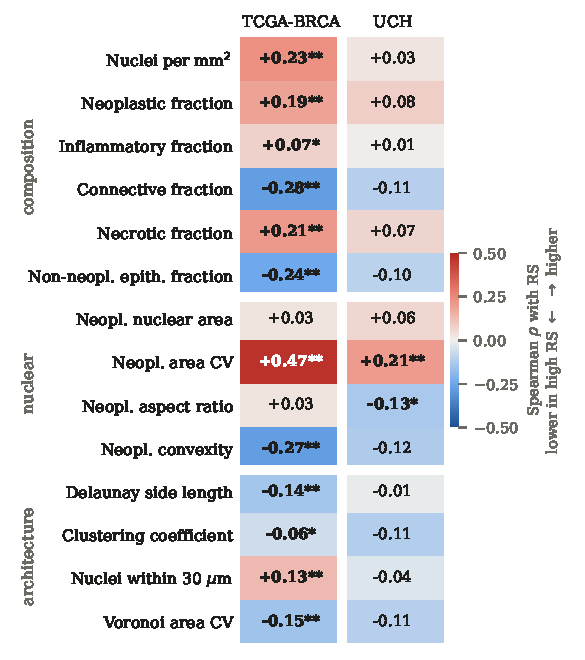
\includegraphics[width=\linewidth]{figures/fig_morph_heatmap_rs.pdf}}
\end{figure}

\subsection{Node Feature Ablation}
\label{sec:node-features}

We also test whether richer node features help, at $N=2$ with the same splits and seeds
(\tableref{tab:nodefeat}). The 13-d base descriptor is compared against three extensions: 32
structural features computed from the nuclear positions in physical units (F1), a 512-d
embedding of an 18\,$\mu$m crop around each nucleus from a frozen ImageNet ResNet-34 (F2), and
both together (F3). The gated model barely moves: on TCGA it goes from 85.1 to 85.4, 84.2 and
84.7, every change within a point. The graph branch alone is more sensitive, and in the
unhelpful direction: F2 lowers its external AUROC from 74.0 to 65.5 on CPTAC-BRCA and from 62.7
to 57.6 on UCH, so a nucleus-level appearance embedding does not transfer across cohorts. We
therefore keep the 13-d features, since nuclear appearance is already covered by the image
branch.

% Data: Dissertation/Results/tables/region_nodefeat_{tcga,external}.csv
% \begin{table}[htbp]
% \floatconts
%   {tab:nodefeat}
%   {\caption{Node feature ablation at $N=2$ (AUROC \%; TCGA: mean $\pm$ SD over folds; external: five-fold ensemble).}}
%   {\small
%   \begin{tabular}{llcccc}
%   \hline
%   Cohort & Model & Base & F1 & F2 & F3 \\
%   \hline
%   TCGA-BRCA  & Graph & 76.2 $\pm$ 3.5 & 76.5 $\pm$ 3.2 & 75.8 $\pm$ 1.3 & 76.6 $\pm$ 1.5 \\
%              & Gated & 85.1 $\pm$ 3.9 & 85.4 $\pm$ 3.7 & 84.2 $\pm$ 4.3 & 84.7 $\pm$ 4.5 \\
%   \hline
%   CPTAC-BRCA & Graph & 74.0 & 76.0 & 65.5 & 68.9 \\
%              & Gated & 78.8 & 78.3 & 77.8 & 78.8 \\
%   \hline
%   UCH        & Graph & 62.7 & 65.5 & 57.6 & 58.3 \\
%              & Gated & 72.7 & 73.5 & 70.9 & 72.2 \\
%   \hline
%   \end{tabular}}
\end{table}

\section{Discussion}
\label{sec:discussion}

% ~1 page

\section{Conclusion}
\label{sec:conclusion}

% ~0.3 pages

\clearpage  % Acknowledgements, references and appendix do not count toward the page limit

% Will not appear in the anonymised version -- MIDL is single-blind, so this is kept.
\midlacknowledgments{}

\bibliography{references}

\appendix

\section{Implementation Details}
\label{app:implementation-details}

\section{Additional Results}
\label{app:additional-results}

\end{document}